\documentclass{article}
\usepackage{caption}
\usepackage{graphicx}
\begin{document}
\fbox{ 
{\centering
\begin{minipage}{.6\textwidth}
  \centering
  
	\begin{center}
	\begin{tabular}{ |c|c| } 
 	\hline
 		No & Items \\ \hline\hline
 		a  & \emph{a(0.9),c(0.6),d(0.5)}\\ \hline
 		b & \emph{a(0.9),b(0.4),e(0.1)}\\ \hline
 		c & \emph{a(0.2),c(0.9),d(0.7)}\\ \hline
 		d & \emph{b(0.3),c(0.9)}\\ \hline
 		dc& \emph{a(0.1),b(0.3),c(0.9)} \\ \hline
 		da & \emph{a(0.9),e(0.3)
}\\ \hline
\end{tabular}
\end{center}  
  
  
  \captionof{table}{Transaction Table after Removing Infrequent Items}
\end{minipage}
\hfill
\begin{minipage}{0.40\textwidth}
  \centering
  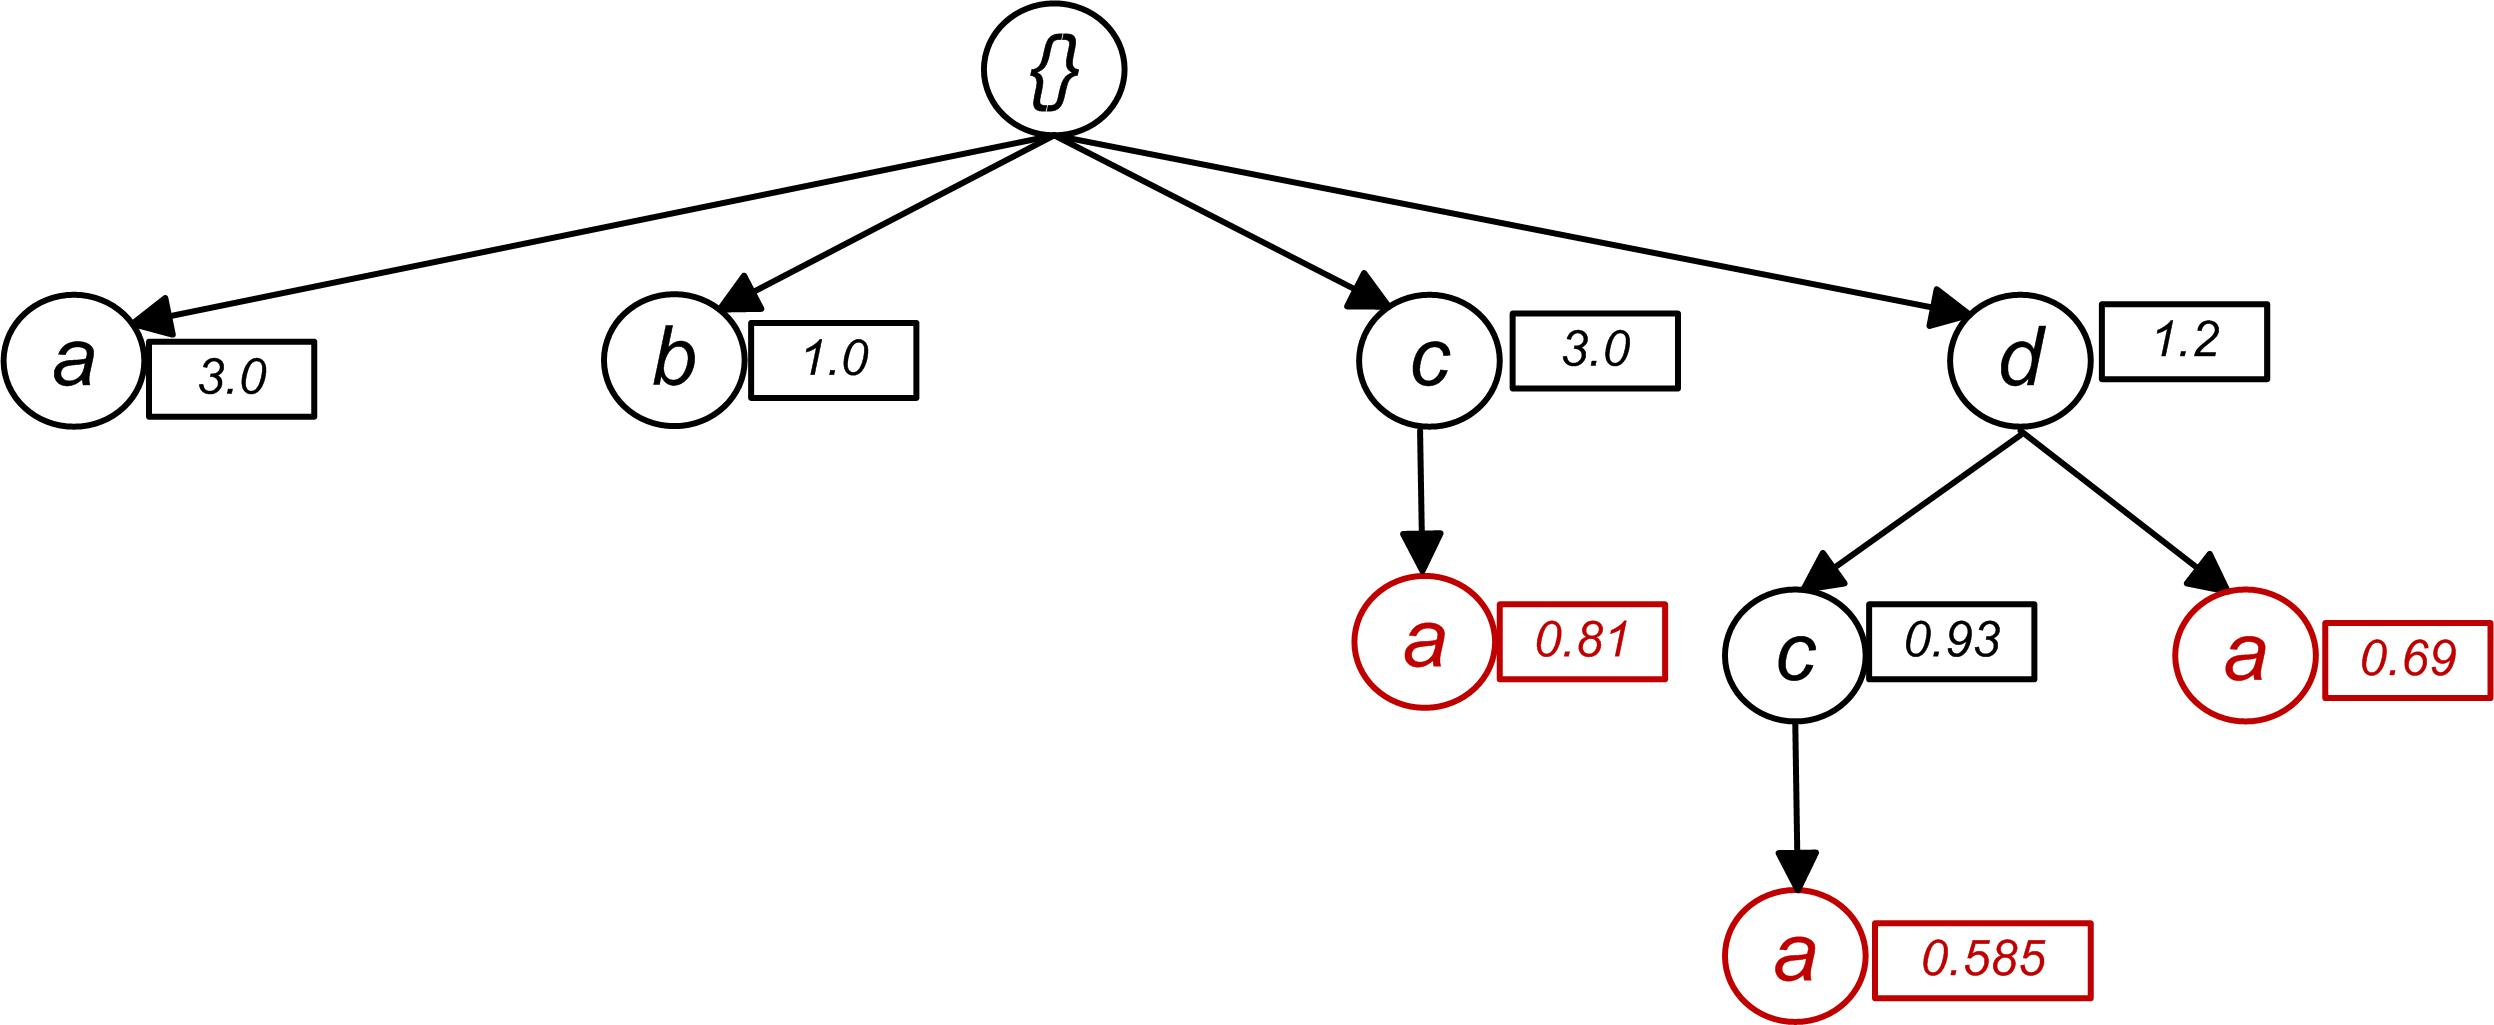
\includegraphics[width=.8\textwidth]{images/frequent_tree_final.jpg}
  \captionof{figure}{Frequent Item Tree Identifying False Positives}
\end{minipage}

}
}

\end{document}